\PassOptionsToPackage{unicode=true}{hyperref} % options for packages loaded elsewhere
\PassOptionsToPackage{hyphens}{url}
\documentclass[11pt,ignorenonframetext,aspectratio=169]{beamer}
\IfFileExists{pgfpages.sty}{\usepackage{pgfpages}}{}
\setbeamertemplate{caption}[numbered]
\setbeamertemplate{caption label separator}{: }
\setbeamercolor{caption name}{fg=normal text.fg}
\beamertemplatenavigationsymbolsempty
\usepackage{lmodern}
\usepackage{amssymb,amsmath}
\usepackage{ifxetex,ifluatex}
\usepackage{fixltx2e} % provides \textsubscript
\ifnum 0\ifxetex 1\fi\ifluatex 1\fi=0 % if pdftex
  \usepackage[T1]{fontenc}
  \usepackage[utf8]{inputenc}
\else % if luatex or xelatex
  \ifxetex
    \usepackage{mathspec}
  \else
    \usepackage{fontspec}
\fi
\defaultfontfeatures{Ligatures=TeX,Scale=MatchLowercase}







\fi

  \usetheme[sectionpage=progressbar, titleformat=regular,
numbering=counter, block=fill]{metropolis}






% use upquote if available, for straight quotes in verbatim environments
\IfFileExists{upquote.sty}{\usepackage{upquote}}{}
% use microtype if available
\IfFileExists{microtype.sty}{%
  \usepackage{microtype}
  \UseMicrotypeSet[protrusion]{basicmath} % disable protrusion for tt fonts
}{}


\newif\ifbibliography
  \usepackage[round]{natbib}
  \bibliographystyle{plainnat}


\hypersetup{
      pdftitle={Genetic composition of cross pollinated populations},
        pdfauthor={Deependra Dhakal},
          pdfborder={0 0 0},
    breaklinks=true}
%\urlstyle{same}  % Use monospace font for urls







% Prevent slide breaks in the middle of a paragraph:
\widowpenalties 1 10000
\raggedbottom

  \AtBeginPart{
    \let\insertpartnumber\relax
    \let\partname\relax
    \frame{\partpage}
  }
  \AtBeginSection{
    \ifbibliography
    \else
      \let\insertsectionnumber\relax
      \let\sectionname\relax
      \frame{\sectionpage}
    \fi
  }
  \AtBeginSubsection{
    \let\insertsubsectionnumber\relax
    \let\subsectionname\relax
    \frame{\subsectionpage}
  }



\setlength{\parindent}{0pt}
\setlength{\parskip}{6pt plus 2pt minus 1pt}
\setlength{\emergencystretch}{3em}  % prevent overfull lines
\providecommand{\tightlist}{%
  \setlength{\itemsep}{0pt}\setlength{\parskip}{0pt}}

  \setcounter{secnumdepth}{0}


  \usepackage{setspace}
  \usepackage{wasysym}
  % \usepackage{fontenc}
  \usepackage{booktabs,siunitx}
  \usepackage{longtable}
  \usepackage{array}
  \usepackage{multirow}
  \usepackage{wrapfig}
  \usepackage{float}
  \usepackage{colortbl}
  \usepackage{pdflscape}
  \usepackage{tabu}
  \usepackage{threeparttable}
  \usepackage{threeparttablex}
  \usepackage[normalem]{ulem}
  \usepackage{makecell}
  \usepackage{xcolor}
  \usepackage{tikz} % required for image opacity change
  \usepackage[absolute,overlay]{textpos} % for text formatting
  \usepackage[skip=0.333\baselineskip]{caption}
  % \usepackage{newtxtext,newtxmath}% better than txfonts   
  \usepackage[english]{babel}
  \usepackage{pgfpages}

  \sisetup{per-mode=symbol}

  % % Added by CII
  % \usepackage[format=hang,labelfont=bf,margin=0.5cm,justification=centering]{caption}
  % \captionsetup{font=small,width=0.9\linewidth,labelfont=small,textfont={small}}
  % % End of CII addition

  % \usepackage{subcaption}
  % \newcommand{\subfloat}[2][need a sub-caption]{\subcaptionbox{#1}{#2}}

  \captionsetup[sub]{font=footnotesize,labelfont=footnotesize,textfont=footnotesize}
  % \captionsetup[subfigure]{font=small,labelfont=small,textfont=small}
  % \captionsetup[subfloat]{font=scriptsize,labelfont=scriptsize,textfont=scriptsize}

  % this font option is amenable for beamer, although these are global settings
  \setbeamerfont{caption}{size=\tiny}
  % \setbeamerfont{subcaption}{size=\tiny} % this does not chage subfloat fonts
  % \setbeamerfont{subfloat}{size=\tiny} % this does not change subfloat fonts
   
   % use single line spacing ?
  \singlespacing

  % use cslreferences environment
  % this is revised as of Oct, 2022 (https://stackoverflow.com/questions/59193797/pandocs-environment-cslreferences-undefined-when-knitting-rmarkdown-to-pdf-in-r)
  \newlength{\cslhangindent}
  \setlength{\cslhangindent}{1.5em}
  \newenvironment{CSLReferences}%
    {\setlength{\parindent}{0pt}%
    \everypar{\setlength{\hangindent}{\cslhangindent}}\ignorespaces}%
    {\par}


  \newcommand{\bcolumns}{\begin{columns}[T, onlytextwidth]}
  \newcommand{\ecolumns}{\end{columns}}

  \newcommand{\bdescription}{\begin{description}}
  \newcommand{\edescription}{\end{description}}

  \newcommand{\bitemize}{\begin{itemize}}
  \newcommand{\eitemize}{\end{itemize}}

  \title[]{Genetic composition of cross pollinated populations}


  \author[
        Deependra Dhakal
    ]{Deependra Dhakal}

  \institute[
    ]{
    Agriculture and Forestry University\\
\textit{ddhakal.rookie@gmail.com}\\
\url{https://rookie.rbind.io}
    }

\date[
      
  ]{
    }


\begin{document}

% Hide progress bar and footline on titlepage
  \begin{frame}[plain]
  \titlepage
  \end{frame}



\hypertarget{meaning-of-population}{%
\section{Meaning of population}\label{meaning-of-population}}

\begin{frame}{}
\protect\hypertarget{section}{}
\begin{itemize}
\tightlist
\item
  A population is a group of sexually interbreeding individuals.
\item
  The capacity to interbreed implies that every gene within the group is
  accessible to all members through the sexual process.
\item
  A gene pool is the total number and variety of genes and alleles in a
  sexually reproducing population that are available for transmission to
  the next generation.
\item
  The genetic structure of a population determines its capacity to be
  changed by selection (i.e., improved by plant breeding)
\item
  The genetic constitution of a population is described by an array of
  gene frequencies.
\item
  The genetic properties of a population are influenced in the process
  of transmission of genes from one generation to the next by four major
  factors - \emph{population size}, \emph{differences in fertility and
  viability}, \emph{migration and mutation}, and the \emph{mating
  system}.
\item
  Breeding of cross-pollinated species tends to focus on population
  improvement rather than individual plants.
\item
  Rather than inheritance of traits, \emph{genetics of population} is
  concerned with how the frequencies of alleles in a gene pool change
  over time.
\end{itemize}
\end{frame}

\hypertarget{breeders-equation-and-response-to-selection}{%
\section{Breeder's equation and response to
selection}\label{breeders-equation-and-response-to-selection}}

\begin{frame}{}
\protect\hypertarget{section-1}{}
\begin{itemize}
\tightlist
\item
  Most phenotypes (occuring in natural environment) show
  \textbf{quantitative}, \textbf{continuous} variation and do not fall
  into discrete classes (understandably, it is not easy to see how
  quantitative traits could arise with mendelian principles).
\end{itemize}

\begin{figure}
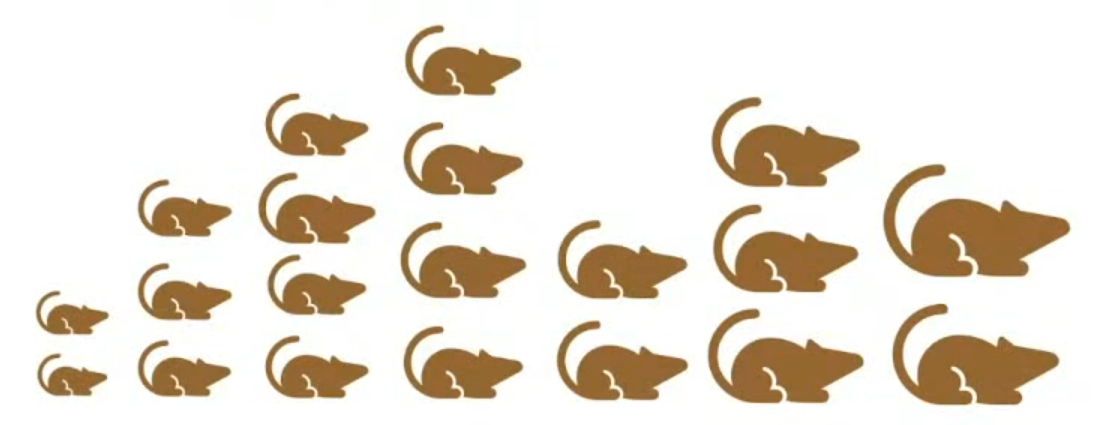
\includegraphics[width=0.65\linewidth]{./images/quantitative_variation} \caption{Body length of mice is a quantitative trait. If we look at a population of mice we see the variation in the trait.}\label{fig:quantitative-variation-mice-size}
\end{figure}
\end{frame}

\begin{frame}{}
\protect\hypertarget{section-2}{}
\begin{columns}
\column{0.35\textwidth}
\begin{itemize}
\item Quantitative traits are controlled by many, many genes.
\item Alleles of each gene that control the trait have small effects (positive or negative) which add up to produce the trait value -- \alert{Infinitesimal model} of quantitative trait inheritance.
\item Each locus that affects the trait is called a quantitative trait locus.
\end{itemize}

\column{0.65\textwidth}


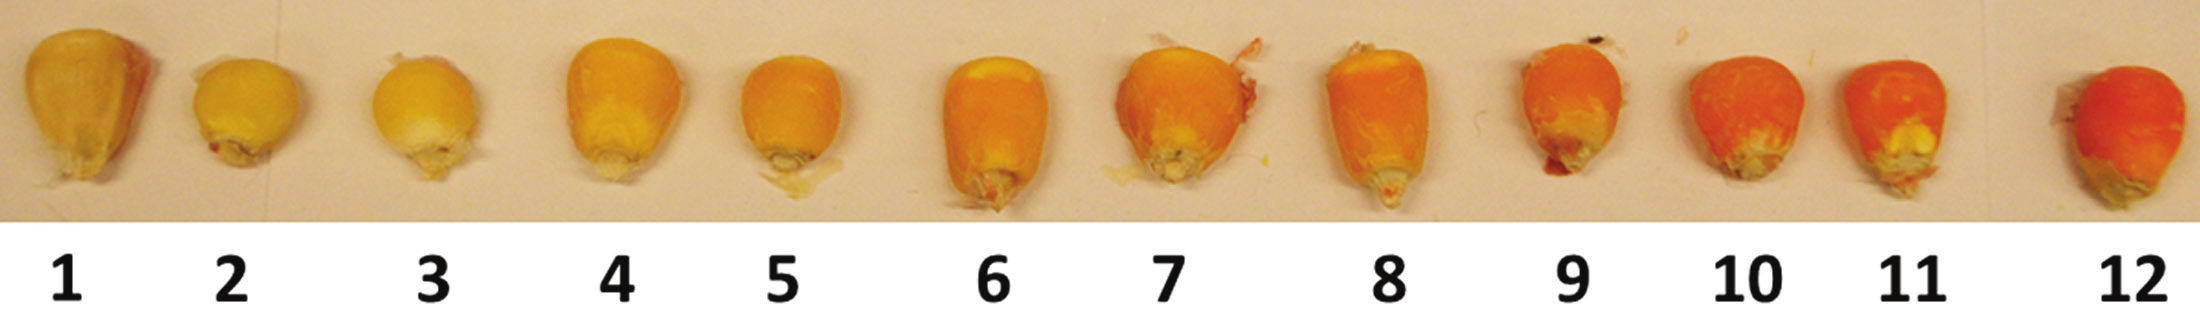
\includegraphics[width=0.8\linewidth]{./images/maize_kernel_color_qtl_study} 

\begin{figure}
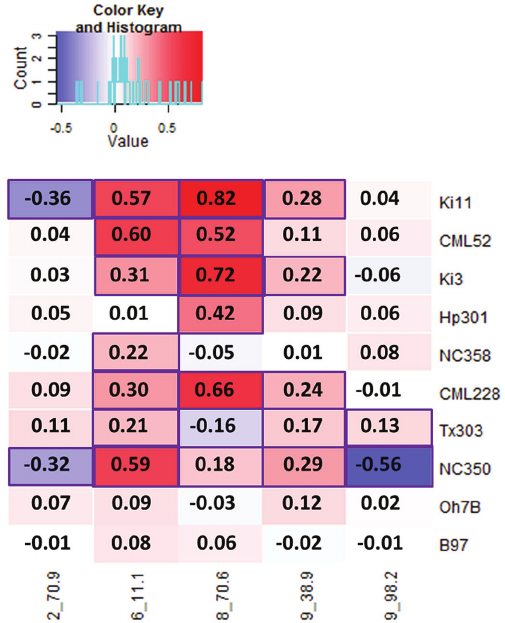
\includegraphics[width=0.5\linewidth]{./images/heatmap-kernel-color-quantitative-trait-loci-QTL-effects-by-chromosome} \caption{Rethinking the genetics of color. Heat map for kernel color quantitative trait loci (QTL) effects by chromosome and position in centimorgans (Chr, cM) and QTL donor. The diverse parents are ordered from highest to lowest kernel color best linear unbiased predictor. The diverse parents with darker orange kernel color tend to have stronger positive effect QTL relative to those with kernels that are yellow or light orange but also have QTL with a moderate-to-weak negative effect. All statistically significant effects at a false discovery rate of 5 percent are indicated by a purple rectangle border. Source: \cite{chandler2013genetic}}\label{fig:heatmap-kernel-color-corn-qtl-chromosome}
\end{figure}

\end{columns}
\end{frame}

\begin{frame}{Breeding for quantitative traits}
\protect\hypertarget{breeding-for-quantitative-traits}{}
\begin{itemize}
\tightlist
\item
  There are too many genes to identify and stack them one by one, we
  need to consider them all at the same time.
\item
  Concentration of favorable alleles and reduction of unfavorable ones
  in a population could be achieved by \textbf{recurrent selection}, all
  while continually picking the best varieties out of what is available.
\item
  Recurrent selection is the engine which drives genetic gain.

  \begin{itemize}
  \tightlist
  \item
    repeatedly extracting superior varieties/cultivars from populations
    is nearly impossible without recurrent selection

    \begin{itemize}
    \tightlist
    \item
      the variance is not enough to overcome the unchanging mean
    \end{itemize}
  \item
    with recurrent selection, repeatedly obtaining superior
    varieties/cultivars are likely
  \end{itemize}
\end{itemize}
\end{frame}

\begin{frame}{}
\protect\hypertarget{section-3}{}
\begin{table}

\caption{\label{tab:probability-of-success-in-recurrent-selection}Probability than an individual superior to all others can be identified every cycle of selection during population improvement. $h^2 = 0$ is equivalent to no population improvement. Source: \cite{rutkoski2019practical}}
\centering
\fontsize{6}{8}\selectfont
\begin{tabular}[t]{rrrrrrrrr}
\toprule
$h^2$ & C2 & C3 & C4 & C5 & C7 & C10 & C15 & C25\\
\midrule
0.00 & 0.58 & 0.17 & 0.07 & 0.01 & 0.00 & 0.00 & 0.00 & 0.00\\
0.10 & 0.54 & 0.34 & 0.29 & 0.14 & 0.12 & 0.11 & 0.12 & 0.16\\
0.20 & 0.66 & 0.44 & 0.33 & 0.34 & 0.28 & 0.28 & 0.31 & 0.28\\
0.25 & 0.66 & 0.47 & 0.37 & 0.36 & 0.41 & 0.36 & 0.34 & 0.29\\
0.40 & 0.70 & 0.60 & 0.56 & 0.49 & 0.53 & 0.46 & 0.46 & 0.50\\
\addlinespace
0.50 & 0.80 & 0.65 & 0.56 & 0.60 & 0.64 & 0.61 & 0.58 & 0.54\\
0.65 & 0.84 & 0.73 & 0.74 & 0.74 & 0.73 & 0.78 & 0.74 & 0.77\\
0.80 & 0.84 & 0.84 & 0.77 & 0.85 & 0.84 & 0.81 & 0.85 & 0.84\\
0.95 & 0.92 & 0.92 & 0.94 & 0.94 & 0.94 & 0.93 & 0.94 & 0.90\\
\bottomrule
\end{tabular}
\end{table}
\end{frame}

\begin{frame}{Response to selection (R)}
\protect\hypertarget{response-to-selection-r}{}
\small

\begin{itemize}
\tightlist
\item
  Selection entails discriminating among genetic variation to identify
  and choose a number of individuals to establish the next generation.
\item
  This results in differential reproduction of genotypes, i.e.~those
  that are selected have chance to increase their gene frequencies.
\item
  Subsequently, the genotypic and phenotypic values of the targeted
  traits also improve.
\item
  By selecting and advancing superior individuals (with high genetic
  potential) from a mixed population, the breeder aims to change
  population mean of the trait in a positive way in the next generation.
\item
  \alert{Response to selection} is the difference between the mean
  phenotypic value of the offspring of the selected parents and the
  whole of the parental generation before selection. It is related to
  \emph{heritability} as shown in the following
  \alert{Breeder's equation}:
\end{itemize}

\bcolumns
\column{0.5\textwidth}

\[
R = \Delta G = h^2 S
\] \column{0.5\textwidth}

\begin{itemize}
\tightlist
\item
  Where,

  \begin{itemize}
  \footnotesize
  \item $R$ is the response to selection
  \item $h^2$ is the heritability of trait ($h^2_{bs}$ or $h^2_{ns}$)
  \item $S$ is the selection differential
  \end{itemize}
\end{itemize}

\ecolumns
\end{frame}

\begin{frame}{Selection differenatial (S)}
\protect\hypertarget{selection-differenatial-s}{}
\begin{itemize}
\tightlist
\item
  \alert{Selection differential (S)} is the mean phenotypic value of the
  individuals selected as parents expressed as a deviation from the
  population mean (i.e., from the mean phenotypic value of all the
  individuals in the parental generation before selection).
\end{itemize}

\[
S = X_s - X_o = i \sigma
\]
\end{frame}

\begin{frame}{}
\protect\hypertarget{section-4}{}
\footnotesize

\begin{itemize}
\tightlist
\item
  Genetic advance achieved through selection depends on three factors:

  \begin{enumerate}
  \footnotesize
  \item Total variation (phenotypic) in the population in which selection will be conducted.
  \item Heritability of the target trait.
  \item Selection pressure to be imposed by the plant breeder (i.e., the proportion of the population that is selected for the next generation).
  \end{enumerate}
\end{itemize}

\[
\Delta_G = \frac{ir\sigma_G}{L}
\]

\begin{itemize}
\tightlist
\item
  Genetic gain is the amount of change in mean genetic value of a
  population over time.

  \begin{itemize}
  \scriptsize
  \item due to selection over breeding (recurrent selection) cycles 
  \item always occurs within a population -- i.e., not the difference between variety and check
  \item sometimes called 'response to selection', denoted R
  \end{itemize}
\item
  Expected genetic gain can be estimated from the breeder's equation,
  although realized genetic gain may differ and can be calculated from
  the observations
\item
  Although it looks relatively simple, the breeder's equation applies to
  every species while breeding for quantitative traits.
\item
  Particular features of the species -- like the age at which plants
  flower, or how quickly genotypes can be replicated -- can influence
  the optimal design of a breeding pipeline.
\end{itemize}
\end{frame}

\begin{frame}{}
\protect\hypertarget{section-5}{}
\bcolumns
\column{0.5\textwidth}

\begin{itemize}
\tightlist
\item
  In principle, the prediction of response is valid for only one
  generation of selection.
\item
  To predict the response in subsequent generations, heritabilities must
  be determined in each generation. Heritabilities are expected to
  change from one generation to the next because, if there is a
  response, it must be accompanied by change in gene frequencies on
  which heritability depends.
\item
  Also, selection of parents tends to reduce phenotypic variance
  especially in early generations.
\end{itemize}

\column{0.5\textwidth}

\begin{figure}

{\centering 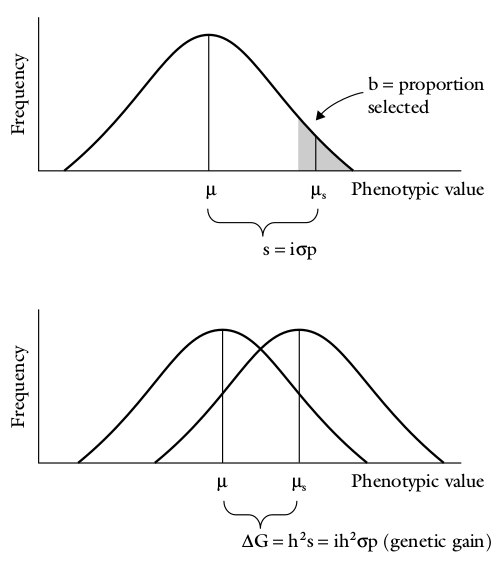
\includegraphics[width=0.7\linewidth]{./images/response_to_selection} 

}

\caption{Genetic gain or genetic advance from selection indicates the progress plant breeders make from one generation to another based on the selection decisions they make.}\label{fig:response-to-selection}
\end{figure}

\ecolumns
\end{frame}

\begin{frame}{Selection intensity}
\protect\hypertarget{selection-intensity}{}
\begin{columns}
\column{0.58\textwidth}
\begin{itemize}
\item Selection intensity ($i$) is the selection differential divided by the phenotypic standard deviation.
  \begin{itemize}
  \item The selection differential ($S$) is the phenotypic deviation of each selected individual from the population mean, divided by the number of selected individuals
  \item The phenotypic standard deviation is just the square root of the phenotypic variance
  \end{itemize}
\item Selection intensity is closely tied to the percentage of individuals selected, especially for normally distributed traits, but is not exactly the same.
  \begin{itemize}
  \item it captures the difference between the selected parents and the overall population
  \end{itemize}
\end{itemize}
\column{0.42\textwidth}

$$
i = \frac{\frac{\sum^n_{i = 1} (y_i - \bar{y})}{n}}{\sigma_p}
$$

$$
\small
S = \frac{\sum^n_{i = 1} (y_i - \bar{y})}{n}
$$


\begin{itemize}
\item Where,
  \begin{itemize}
    \footnotesize
    \item $i$: Selection intensity
    \item $S$: Selection differential
    \item $y_i$: Phenotypic value of the $\mathrm{i^{th}}$ selected individuals
    \item $\bar{y}$: Mean phenotypic value of all individuals in the population
    \item $n$: Number of selected individuals
    \item $\sigma_P$: Phenotypic standard deviation among all individuals in the population
    \end{itemize}
  \end{itemize}
  
\end{columns}
\end{frame}

\begin{frame}{}
\protect\hypertarget{section-6}{}
\footnotesize

For a quantitative trait in RMP, mean is 100 and variation is 240. The
regression of the offspring on mid-parent value is 0.25. Truncation
selection is practiced with a selection differential of 32. What is the
expected mean in the next generation ?

\(\longrightarrow\)

\begin{itemize}
\footnotesize
\item Mean ($X_0$) = 100
\item Variation ($\sigma^2$) = 240
\item Regression of offspring on mid-parent value ($b$) = 0.25
\item Selection differential ($X_s - X_0$) = 32
\end{itemize}

We know that the performance of a selected population after applying
selection differential:

\begin{align}
\small
S &= \sqrt{\sigma^2} i = \sqrt{240} i \notag \\
i &= \frac{S}{\sqrt{240}} \notag
\end{align}

\(\therefore\) \(i\) = 2.07. And we know that \(b = h^2_{ns}\), so:

\(\rightarrow\) \(R = \sigma i h^2\) = 8

Hence, the expected mean of next (progeny) generation (\(P\)) =
\(X_0 + \sigma i h^2\) = 108.
\end{frame}

\hypertarget{hardy-weinberg-law}{%
\section{Hardy-weinberg law}\label{hardy-weinberg-law}}

\begin{frame}{}
\protect\hypertarget{section-7}{}
\begin{itemize}
\tightlist
\item
  The genetic constitution of individuals in a population is
  reconstituted for each subsequent generation whereas the genes carried
  by the population have continuity from one generation to the next.
\item
  Plant breeders often work with genetic phenomena in populations that
  exhibit no apparent Mendelian segregation, even though in actuality,
  they obey Mendelian laws.
\item
  Mendel worked with genes whose effects were categorical (kinds) and
  were readily classifiable (ratios) into kinds in the progeny of
  crosses.
\item
  Breeders, on the other hand, are usually concerned about differences
  in populations measured in degrees rather than kinds.
\item
  Population genetics uses mathematical models to attempt to describe
  population phenomena. It is, thus, necessary to make assumptions about
  the population and its environment.
\end{itemize}
\end{frame}

\begin{frame}{Calculating gene frequency}
\protect\hypertarget{calculating-gene-frequency}{}
\begin{itemize}
\item
  Gene frequencies are simply the proportions of the different alleles
  of a gene in a population.
\item
  To obtain these proportions we count the total number of organisms
  with various genotypes in the population and estimate the relative
  frequencies of the alleles involved.
\item
  To understand the genetic structure of population, consider a large
  population in which random mating occurs, with no mutation or gene
  flow between this population and others, no selective advantage for
  any genotype, and normal meiosis.
\item
  Consider also one locus, \(A\), with two alleles, \(A\) and \(a\). The
  frequency of allele \(A_1\), in the gene pool is \(p\), while the
  frequency of allele \(A_2\) is \(q\). Also, \(p + q = 1\) (or 100\% of
  the gene pool). Assume a population of \(N\) diploids in which two
  alleles ( \(A\), \(a\)) occur at one locus.
\item
  Assuming dominance at the locus, three genotypes -- \(AA\), \(Aa\) and
  \(aa\) -- are possible in an \(F_2\) segregating population. Assume
  the genotypic frequencies are \(D\) (for \(AA\)), \(H\) (for \(Aa\))
  and \(Q\) (for \(aa\)). Since the population is diploid, there will be
  \(2N\) alleles in it. The genotype \(AA\) has two \(A\) alleles.
  Hence, the total number of \(A\) alleles in the population is
  calculated as \(2D + H\). The proportion or frequency of \(A\) alleles
  (designated as \(p\)) in the population is obtained as follows.
\end{itemize}

\[
\begin{aligned}
\frac{2D + H}{2N} = D + \frac{1}{2}H = p
\end{aligned}
\]

The same can be done for allele \(a\), and designated \(q\). Further,
\(p + q = 1\) and hence \(p = 1-q\).
\end{frame}

\begin{frame}{Numerical example}
\protect\hypertarget{numerical-example}{}
If \(N = 80\), \(D = 4\) and \(H = 24\). (Here, D and H are rather used
as count of individuals rather than frequencies)

Genotypic frequencies;

\[
\begin{aligned}
D = 4/80 \\
H = 24/80 \\
Q = 52/80
\end{aligned}
\] Now,

\[
p = \frac{D + \frac{1}{2}H}{N} = \frac{4 + 12}{80} = \frac{16}{80} = 0.2
\]

Since \(p + q = 1\), \(q = 1-p\), and hence \(q = 1-0.2 = 0.8\).
\end{frame}

\begin{frame}{HW Equilibrium}
\protect\hypertarget{hw-equilibrium}{}
\begin{itemize}
\tightlist
\item
  Consider a random mating population (each male gamete has an equal
  chance of mating with any female gamete).
\item
  Random mating involving the previous locus (A/a) will yield the
  following genotypes: \(AA\), \(Aa\), and \(aa\), with the
  corresponding frequencies of \(p^2+2pq+q^2\), respectively.
\item
  The gene frequencies must add up to the unity. Consequently,
  \(p^2+2pq+q^2 = 1\). This mathematical relationship is called
  Hardy-Weinberg equilibrium.
\item
  Hardy, from England, and Weinberg, from Germany, discovered that
  equilibrium between genes and genotypes is achieved in large
  populations.
\item
  They showed that the frequency of genotypes in a population depends on
  the frequency of genes in the preceding generation, not on the
  frequency of the genotypes.
\end{itemize}
\end{frame}

\begin{frame}{}
\protect\hypertarget{section-8}{}
Considering the previous example, the genotypic frequencies for the next
generation following random mating can be calculated as follows:

\[
\begin{aligned}
AA &= p^2 &= 0.2^2 &= 0.04 \\
Aa &= 2pq &= 2 (0.2\times0.8) &= 0.32 \\
aa &= q^2 &= 0.8^2 &= 0.64
\end{aligned}
\]

\begin{itemize}
\tightlist
\item
  The Hardy-Weinberg equilibrium is hence summarized as:
\end{itemize}

\[
p^2AA + 2pqAa + q^2aa = 1
\]
\end{frame}

\begin{frame}{}
\protect\hypertarget{section-9}{}
\begin{itemize}
\tightlist
\item
  This means that in a population of 80 plants as before, about three
  plants will have a genotype of \(AA\), 26 will be \(Aa\), and 51,
  \(aa\). Using the previous formula, the frequencies of the genes in
  the next generation may be calculated as:
\end{itemize}

\[
P = \frac{D + \frac{1}{2} H}{N} = \frac{3+13}{80} = 0.2
\]

And, \(q = 1-p = 0.8\)

\begin{itemize}
\tightlist
\item
  The allele frequencies have remained unchanged, while the genotypic
  frequencies have changed (for AA, Aa, and aa, respectively) from 4,
  24, and 52, to 3, 26, and 51.
\item
  However, in subsequent generations, both the genotype and gene
  frequencies will remain unchanged, provided that:

  \begin{itemize}
  \tightlist
  \item
    Random mating occurs in a very large diploid population;
  \item
    Allele \(A\) and allele \(a\) are equally fit (one does not confer a
    superior trait than the other);
  \item
    There is no differential migration of one allele into or out of the
    population;
  \item
    The mutation rate of allele \(A\) is equal to that of allele \(a\).
  \end{itemize}
\end{itemize}
\end{frame}

\hypertarget{changing-gene-and-genotypic-frequencies-in-hw-population}{%
\section{Changing gene and genotypic frequencies in HW
population}\label{changing-gene-and-genotypic-frequencies-in-hw-population}}

\begin{frame}{}
\protect\hypertarget{section-10}{}
\begin{figure}[center]
\includegraphics[width=0.68\linewidth]{08-genetic_composition_of_cross_pollinated_populations_pdf_files/figure-beamer/hw-expectation-in-frequencies-1} \caption{Attainment of HW-equilibrium in a diploid population shown across different values of starting allele frequencies (An example scenario with starting allele frequencies f(A) = 0.2 and f(a) = 0.8 is shown as marked.)}\label{fig:hw-expectation-in-frequencies}
\end{figure}

The relationship between allele frequencies and genotype frequencies in
a population in Hardy--Weinberg equilibrium for two alleles. The
frequency of the heterozygotes cannot be more than 50\%, and this
maximum occurs when the allele frequencies are \(p=q=0.5\). Further,
when the frequency of an allele is low, the rare allele occurs
predominantly in heterozygotes and there are very few homozygotes.
(Adapted from Falconer, 1981.)
\end{frame}

\begin{frame}{Summary of HW principle}
\protect\hypertarget{summary-of-hw-principle}{}
\begin{itemize}
\tightlist
\item
  Hence the stability of genotypic frequency after the first generation
  is said to be in equilibrium.
\item
  This genotypic equilibrium, based on stable gene frequencies and
  random mating, is known as Hardy-Weinberg principle (or law)
\item
  Hence, Genetic differences in a randomly breeding population will tend
  to remain constant unless acted upon by external forces.
\item
  In other words, the variability does not change from one generation to
  another in a random mating population.
\item
  The maximum frequency of the heterozygote (H) cannot exceed 0.5. The
  Hardy-Weinberg law states that equilibrium is established at any locus
  after one generation of random mating.
\end{itemize}
\end{frame}

\begin{frame}{Plant Breeding implications of HW principle}
\protect\hypertarget{plant-breeding-implications-of-hw-principle}{}
\begin{itemize}
\tightlist
\item
  From the standpoint of plant breeding, two states of variability are
  present -- two homozygotes (AA, aa), called ``free variability'' that
  can be fixed by selection and the intermediate heterozygous (Aa),
  called ``hidden or potential variability, that can generate new
  variability through segregation.
\item
  In outcrossing species, the homozygotes can hybridize to generate more
  heterozygotic variability. Under random mating and no selection, the
  rate of crossing and segregation will be balanced to maintain the
  proportion of free and potential variability of 50\%:50\%.
\item
  However, with two loci under consideration, equilibrium will be
  attained slowly over many generations.
\item
  If genetic linkage is strong, the rate of attainment of equilibrium
  will be even much slower.
\end{itemize}
\end{frame}

\begin{frame}{Plant Breeding application of HW principle}
\protect\hypertarget{plant-breeding-application-of-hw-principle}{}
\begin{itemize}
\tightlist
\item
  In disease resistance breeding, plant breeders cross an elite
  susceptible cultivar with one that has disease resistance. Consider a
  cross between two populations, susceptible x resistant. If the gene
  frequencies of an allele \(A\) in the two populations are represented
  by \(P_1\) and \(P_2\), the gene frequency in the
  \(F_1 = \frac{P_1 + P_2}{2} = p\). Assuming the frequency of the
  resistance gene (Note here that same allele is being considered) in
  the resistant cultivar is \(P_1=0.7\) and that in the susceptible
  elite cultivar is \(P_2=0.05\), the gene frequency in the progeny of
  the cross p would be obtained as follows:
  \(p = \frac{P_1 + P_2}{2} = (0.7 + 0.05)/2 = 0.375\)
\item
  Consequently, the gene frequency for the resistant trait is reduced by
  about 50\% (from 0.7 to 0.375).
\end{itemize}
\end{frame}

\hypertarget{forces-changing-gene-frequencies}{%
\section{Forces changing gene
frequencies}\label{forces-changing-gene-frequencies}}

\begin{frame}{Mutation}
\protect\hypertarget{mutation}{}
\begin{itemize}
\tightlist
\item
  Introduces a particular gene into a population
\item
  A unique mutation (non-recurrent mutation) would have little impact on
  gene frequencies.
\item
  Types: forward and reverse mutation (Based on the direction of
  mutation)

  \begin{itemize}
  \tightlist
  \item
    Wild type (A) \(\rightarrow\) Mutant type (a)
  \item
    Mutant type (a) \(\rightarrow\) Wild type (A)
  \end{itemize}
\item
  Even if the rate of mutation of A to a is small, after a large number
  of generations, A will disappear.
\end{itemize}
\end{frame}

\begin{frame}{Selection and fitness}
\protect\hypertarget{selection-and-fitness}{}
\begin{itemize}
\tightlist
\item
  One of the most important causes for the change in gene frequency lies
  in the ability of its carriers to produce surviving offspring.
\item
  If individuals carrying gene A are more successful in reproduction,
  than those carrying a, the frequency of former tends to be greater
  than the latter.
\item
  Wide variety of mechanisms responsible for reproductive success of a
  genotype is known collectively as \emph{selection}.
\item
  Artificial and Natural selection
\item
  \emph{Fitness} has a variety of applied meanings, but generally refer
  to ability and aptitude.
\item
  In genetic sense, it is far more restricted to relative reproduction
  success.
\item
  Whether a genotype appears superficially ``weak'' or ``strong'',
  ``beautiful'' or ``ugly'', may be of no matter, only when a genotype
  can produce more offspring than another in the same environment, is
  its fitness superior.
\end{itemize}
\end{frame}

\begin{frame}{Migration}
\protect\hypertarget{migration}{}
\begin{itemize}
\tightlist
\item
  A population may receive alleles by migration from a nearby population
  that maintains an entirely different gene frequency.
\item
  Two factors are important for recipient population in this case:

  \begin{itemize}
  \tightlist
  \item
    The difference in frequencies between the two populations and
  \item
    The proportions of migrant genes that are incorporated each
    generation
  \end{itemize}
\end{itemize}
\end{frame}

\begin{frame}{Random genetic drift}
\protect\hypertarget{random-genetic-drift}{}
\small

\begin{itemize}
\tightlist
\item
  When unopposed the previously discussed forces (Mutation, selection
  and migration) can lead of fixation of one allele and elimination of
  all others, or, when balanced, they can lead to equilibrium between
  two or more alleles.
\item
  However, Random genetic drift is one of the most important
  non-directional forces that arises from variable sampling of the gene
  pool each generation and is known as random genetic drift.
\item
  Genetic drift is caused by the fact that real populations are limited
  in size rather than infinite, so that gene-frequency changes occur
  because of sampling errors.
\item
  Example: If only a few parents are chosen to begin a new generation,
  such a small sample of genes may deviate widely from the gene
  frequency of the previous generation.
\end{itemize}

\begin{center}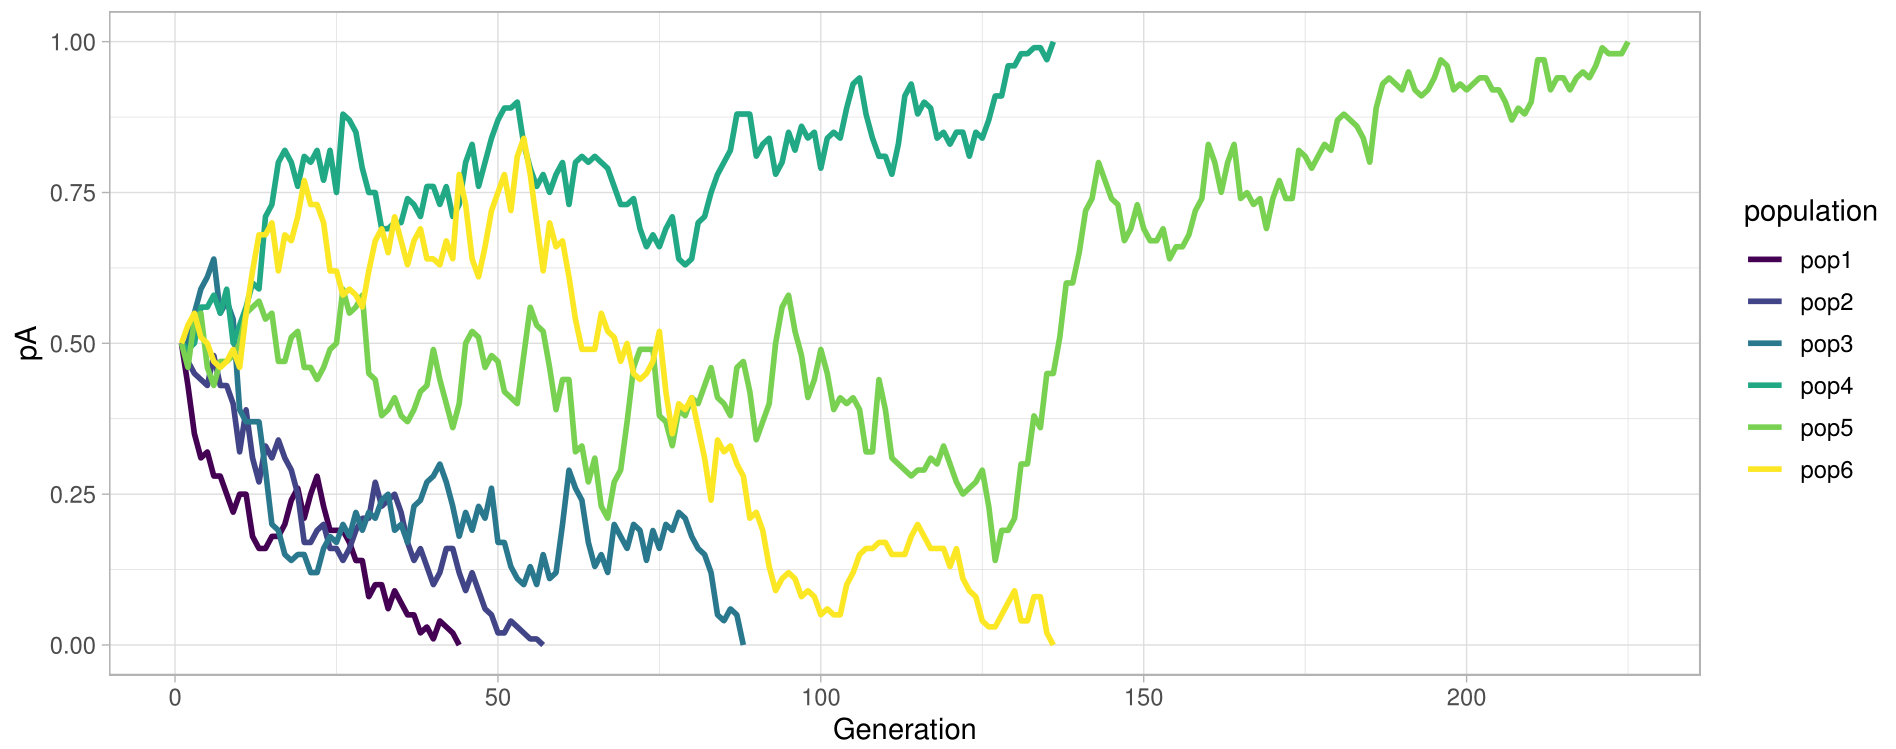
\includegraphics[width=0.54\linewidth]{./images/genetic_drift_simulation} \end{center}
\end{frame}

\begin{frame}{Mating systems}
\protect\hypertarget{mating-systems}{}
\bcolumns
\column{0.44\textwidth}

\small

\begin{itemize}
\tightlist
\item
  Equilibrium assumption is violated if the probability of mating
  depends on a phenotype encoded by a particular genotype at a locus.

  \begin{itemize}
  \footnotesize
  \item Individuals with similar phenotype mate -- assortative mating
  \item Individuals with dissimilar phenotypes mate -- negative or disassortative mating.
  \end{itemize}
\item
  Positive assortative mating on the basis of phenotype can create an
  excess of homozygotes.
\item
  Disassortative mating is common in many fungi, algae and protozoans,
  in which gametes of the same species can only fuse to form zygote if
  they differ in mating type.
\end{itemize}

\column{0.56\textwidth}

\begin{figure}
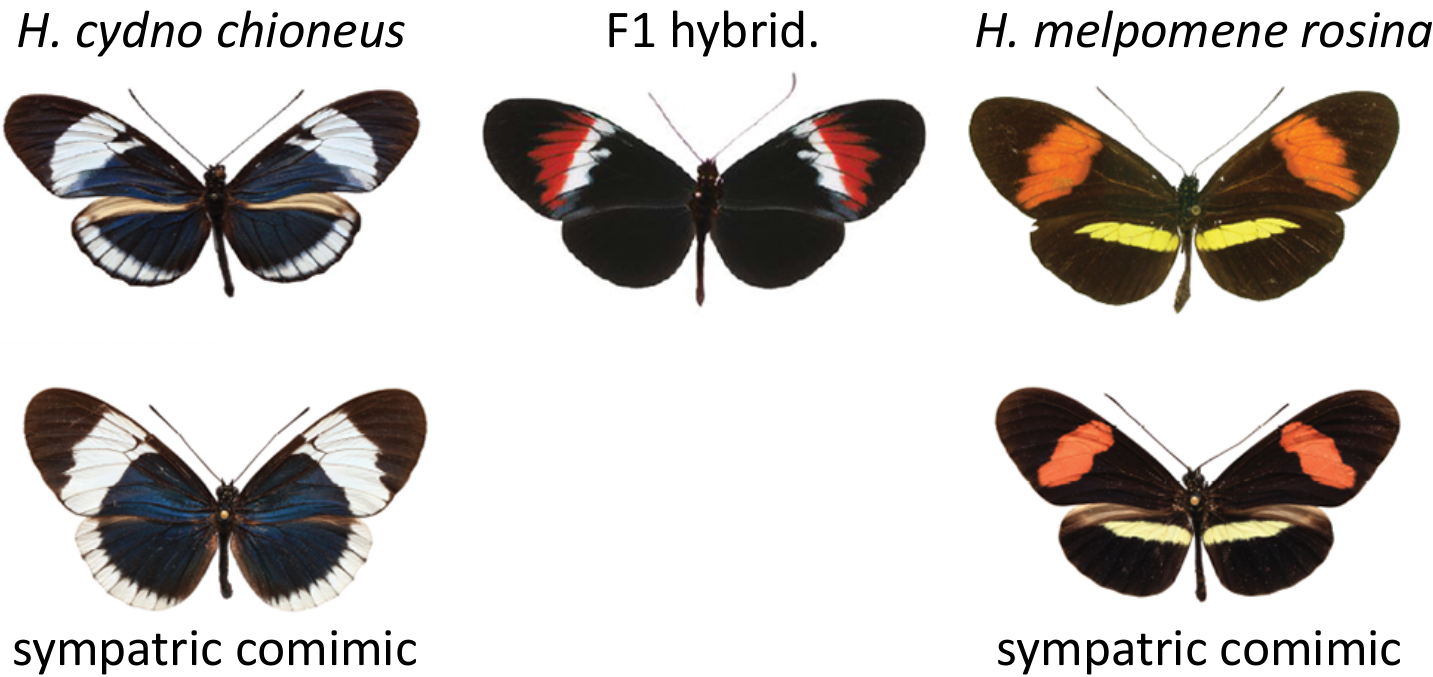
\includegraphics[width=0.72\linewidth]{./images/assortative_mating} \caption{Wing pattern phenotypes of Helconius butterfly. These butterflies are famous for their mimicry, where poisonous pairs of distantly related species mimic each others' bright colour patterns and so share the benefits of being avoided by visual predators (Mullerian mimics). \textit{H. melpomene rosina} and \textit{H. cydno chioneus} are closely related species that co-occur in central Panama, but mimic different other co-occuring species. These differences in coloration pattern are due to a few large effect loci. The two species can hybridize and produce viable F1 hybrids. These F1 hybrids are heterozygote at color loci and their intermediate appearance mean that they're poor mimics and so are quickly eaten by predators. However, these heterozygote (F1) hybrids are very rare in nature $\frac{1}{1000}$ as the parental species show strong positive assortative mating based on color pattern, based on genetic differences in mate preference.}\label{fig:assortative-mating}
\end{figure}

\ecolumns
\end{frame}

\hypertarget{bibliography}{%
\section{Bibliography}\label{bibliography}}

\begin{frame}{References}
\protect\hypertarget{references}{}
\end{frame}

          \begin{frame}[allowframebreaks]{}
    \bibliographytrue
    \bibliography{./../bibliographies.bib}
    \end{frame}
  


\end{document}
